%% ============================================================
%% preamble.tex — 용산 글모음 (어린이 그림책 판)
%% XeLaTeX 으로 컴파일한다
%% ============================================================

%% ----- 한국어 -----
\usepackage{kotex}

%% ----- 폰트 -----
%% 어린이 책이므로 본문을 돋움(고딕)으로 두어 획이 단순하고 크게 보이도록 한다.
%% 시 본문만 바탕(명조)으로 두어 결이 다르게 읽히게 한다.
\usepackage{fontspec}
\defaultfontfeatures{Mapping=}          %% KoPub 에 en/em-dash 글리프가 없다

\setmainfont{KoPubDotum}[
  Scale=1.0, Mapping=,
  BoldFont = {KoPubDotum Bold}
]
\setsansfont{KoPubDotum}[Scale=1.0, Mapping=, BoldFont={KoPubDotum Bold}]

\setmainhangulfont{KoPubDotum}[Scale=1.0, Mapping=, BoldFont={KoPubDotum Bold}]
\setsanshangulfont{KoPubDotum}[Scale=1.0, Mapping=, BoldFont={KoPubDotum Bold}]

\newfontfamily\bookserif{KoPubBatang}[Scale=1.0, Mapping=, BoldFont={KoPubBatang Bold}]
\newhangulfontfamily\bookserifhangul{KoPubBatang}[Scale=1.0, Mapping=, BoldFont={KoPubBatang Bold}]
\newfontfamily\booklight{KoPubDotum Light}[Scale=1.0, Mapping=]
\newhangulfontfamily\booklighthangul{KoPubDotum Light}[Scale=1.0, Mapping=]

%% 대시·불릿은 KoPub 에 없으므로 라틴 폰트로 대신한다
\newfontfamily\latinfont{Times New Roman}[Scale=1.0]
\usepackage{newunicodechar}
\newunicodechar{–}{{\latinfont\char"2013}}
\newunicodechar{—}{{\latinfont\char"2014}}
\newunicodechar{…}{{\latinfont\char"2026}}
\newunicodechar{·}{{\latinfont\char"00B7}}
\newunicodechar{•}{{\latinfont\char"2022}}

%% ----- 판형 -----
%% 어린이 그림책에 흔한 큼직한 정사각에 가까운 판형 (200 x 250 mm)
\usepackage{geometry}
\geometry{
  paperwidth=200mm, paperheight=250mm,
  top=20mm, bottom=22mm,
  inner=20mm, outer=18mm,
  headheight=14pt, headsep=7mm,
  footskip=14mm
}

%% ----- 색 -----
%% 사이트와 같은 주황을 중심에 두고, 그림의 수채 느낌에 맞는 부드러운 색을 곁들인다
\usepackage{xcolor}
\definecolor{ysorange}{HTML}{FA5D29}     % 주조색 — 사이트 액센트
\definecolor{ysink}{HTML}{2E2A26}        % 본문 잉크 (완전한 검정보다 따뜻하게)
\definecolor{yssoft}{HTML}{6E6259}       % 보조 글씨
\definecolor{yspaper}{HTML}{FFFCF6}      % 종이 바탕 (아주 옅은 크림)
\definecolor{yscream}{HTML}{FDF3E7}      % 상자 바탕
\definecolor{ysgreen}{HTML}{6BA368}      % 자연 — 초록
\definecolor{ysblue}{HTML}{5B8FB9}       % 기억 — 하늘
\definecolor{ysplum}{HTML}{A2678A}       % 가족 — 자두
\definecolor{ysgold}{HTML}{D9A441}       % 황혼 — 금빛
\definecolor{ysline}{HTML}{E6DED2}       % 얇은 선

\pagecolor{yspaper}
\color{ysink}

%% ----- 그림 -----
\usepackage{graphicx}
\graphicspath{{images/}{../assets/book/}{../assets/view/}}

\usepackage{tikz}
\usetikzlibrary{calc}

\usepackage[most]{tcolorbox}

%% ----- 줄간격 -----
%% 줄 사이는 곳곳에서 \fontsize{크기}{줄간격} 으로 직접 정한다.
%% 그래서 여기서는 배수를 1로 두어 두 번 곱해지지 않게 한다.
\linespread{1.0}
\setlength{\parskip}{0.75em}
\setlength{\parindent}{0pt}
\raggedbottom

%% 한글은 낱말 단위로 줄을 바꿔야 읽기 쉽다
\usepackage{ragged2e}

%% ----- 머리말·꼬리말 -----
\usepackage{fancyhdr}
\usepackage{lastpage}

%% 쪽 번호는 바깥쪽 아래에 동그란 딱지로 (아이가 쪽을 찾기 쉽게)
\newcommand{\pagebadge}[1]{%
  \tikz[baseline=(n.base)]{
    \node[circle, fill=ysorange, text=white, inner sep=0pt,
          minimum size=8.4mm, font=\sffamily\bfseries\fontsize{11}{11}\selectfont] (n) {#1};
  }%
}

\fancypagestyle{ysmain}{%
  \fancyhf{}
  \renewcommand{\headrulewidth}{0pt}
  \renewcommand{\footrulewidth}{0pt}
  \fancyfoot[LE]{\pagebadge{\thepage}}
  \fancyfoot[RO]{\pagebadge{\thepage}}
}
\fancypagestyle{ysplain}{%
  \fancyhf{}
  \renewcommand{\headrulewidth}{0pt}
  \renewcommand{\footrulewidth}{0pt}
}
\pagestyle{ysmain}

%% ----- 제목 모양 -----
\usepackage{titlesec}

%% 차례의 쪽 번호 칸 — 세 자리가 들어가도 넘치지 않게 넓힌다
\makeatletter
  \renewcommand{\@pnumwidth}{2.6em}
  \renewcommand{\@tocrmarg}{3.4em}
\makeatother

%% ----- 링크 (PDF 목차) -----
\usepackage[hidelinks, bookmarks=true, bookmarksnumbered=false]{hyperref}
\hypersetup{
  pdftitle={용산 글모음},
  pdfauthor={강양수},
  pdfsubject={시와 자서전},
  pdflang={ko}
}

%% ============================================================
%% 책을 이루는 조각들
%% ============================================================

%% ----- 그림 한 장 -----
%% 모서리를 둥글게 깎는다. 세로 그림도 가로 그림도 그대로 받는다.
\newcommand{\ysart}[2][\linewidth]{%
  \begin{center}
    \begin{tikzpicture}
      \node[inner sep=0pt, rounded corners=3.2mm, clip] (img)
        {\includegraphics[width=\dimexpr#1-1pt\relax]{#2}};
      \draw[rounded corners=3.2mm, ysline, line width=0.6pt]
        (img.south west) rectangle (img.north east);
    \end{tikzpicture}
  \end{center}%
}

%% 판면에 가득 차는 그림 (가로·세로 어느 쪽이 걸리든 넘치지 않게)
\newcommand{\ysfullart}[1]{%
  \begin{tikzpicture}
    \node[inner sep=0pt, rounded corners=3.6mm, clip] (img)
      {\includegraphics[width=\dimexpr\linewidth-1pt\relax,
                        height=\dimexpr\textheight-1pt\relax,
                        keepaspectratio]{#1}};
    \draw[rounded corners=3.6mm, ysline, line width=0.6pt]
      (img.south west) rectangle (img.north east);
  \end{tikzpicture}%
}

%% 그림만으로 한 면을 채운다 (판면 한가운데에 정확히 앉힌다)
\newcommand{\ysartpage}[1]{%
  \thispagestyle{ysplain}%
  \begingroup
    \parindent=0pt \parskip=0pt
    \setbox0=\hbox{\ysfullart{#1}}%
    \vbox to \textheight{\vfil\hbox to \linewidth{\hss\box0\hss}\vfil}%
  \endgroup
  \clearpage
}

%% ----- 앞표지 -----
%% 그림을 종이 끝까지 채우고, 그 위에 제목 판을 얹는다.
%% (그림이 종이보다 세로로 길어 폭에 맞추면 위아래가 조금 잘린다 — 그림책에서 흔한 방식)
\newcommand{\yscoverpage}[3]{% {작은 글씨}{제목}{지은이}
  \thispagestyle{ysplain}%
  \begin{tikzpicture}[remember picture, overlay]
    \begin{scope}
      \clip (current page.south west) rectangle (current page.north east);
      \node[inner sep=0pt] at (current page.center)
        {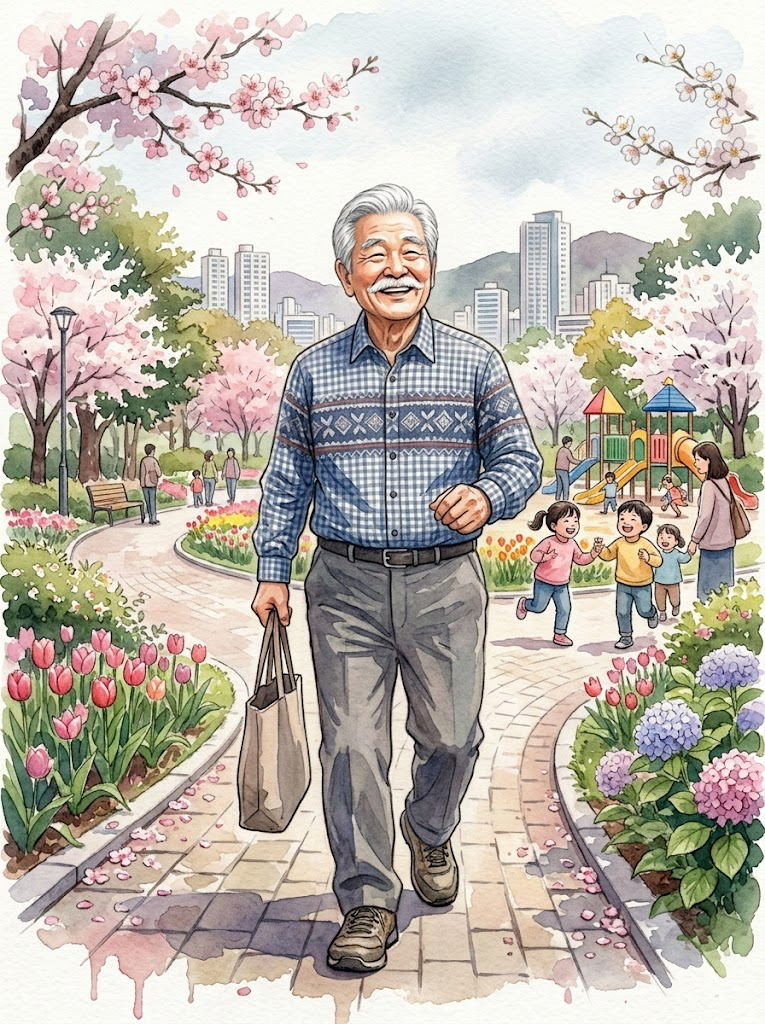
\includegraphics[width=\paperwidth]{001.jpg}};
    \end{scope}
    \node[anchor=south, inner sep=0pt] at ([yshift=18mm]current page.south) {%
      \begin{tcolorbox}[
        enhanced, width=0.80\paperwidth,
        colback=yspaper, colframe=yspaper,
        arc=4mm, boxrule=0pt,
        left=8mm, right=8mm, top=8mm, bottom=8mm,
        drop shadow={black!45, opacity=0.25},
      ]
        \centering
        {\sffamily\bfseries\fontsize{12}{14}\selectfont\color{ysorange} #1\par}
        \vspace{4mm}
        {\sffamily\bfseries\fontsize{36}{42}\selectfont\color{ysink} #2\par}
        \vspace{5mm}
        {\color{ysorange}\rule{28mm}{1.8pt}\par}
        \vspace{5mm}
        {\sffamily\fontsize{14}{17}\selectfont\color{yssoft} #3\par}
      \end{tcolorbox}%
    };
  \end{tikzpicture}%
  \null
  \clearpage
}

%% ----- 이야기 한 자락이 늘 홀수 쪽에서 시작하도록 맞춘다 -----
%% 홀수 쪽에 그림, 이어지는 짝수 쪽에 글이 온다.
%% 이미 홀수 쪽이면 그냥 두고, 짝수 쪽이면 한 장을 비워 홀수로 넘긴다.
\newcommand{\ysensurerecto}{%
  \clearpage
  \ifodd\value{page}\else\hbox{}\thispagestyle{ysplain}\clearpage\fi
}

%% ----- 이야기 한 자락 -----
%% 왼쪽 면에 그림 한 장 가득, 마주 보는 오른쪽 면에 글.
%% 그림책에서 아이가 그림을 먼저 보고 글을 듣는 순서 그대로다.
\newenvironment{storypage}[1]% {그림파일}
  {\ysensurerecto
   \ysartpage{#1}%
   \begingroup
   \vspace*{\fill}
   \fontsize{15}{28}\selectfont\RaggedRight}
  {\vspace*{\fill}\endgroup\clearpage}

%% ----- 노랫말·인용 -----
\newcommand{\ysverse}[1]{%
  \begin{center}
  \begin{tcolorbox}[
    enhanced, width=0.92\linewidth,
    colback=yscream, colframe=yscream,
    arc=3mm, boxrule=0pt,
    borderline west={1.6mm}{0mm}{ysorange},
    left=7mm, right=5mm, top=5mm, bottom=5mm,
  ]
  \begingroup\bookserifhangul\fontsize{13}{21}\selectfont\color{ysink}
  #1
  \endgroup
  \end{tcolorbox}
  \end{center}%
}

%% ----- 부 표지 -----
%% 그림은 장(챕터)마다 따로 있으므로, 부 표지는 글자만으로 조용히 연다
\newcommand{\yspart}[3]{% {작은 글씨}{제목}{차례에 적을 이름}
  \ysensurerecto
  \phantomsection
  \addcontentsline{toc}{chapter}{#3}
  \thispagestyle{ysplain}
  \begingroup
  \centering
  \vspace*{\fill}
  {\sffamily\bfseries\fontsize{14}{17}\selectfont\color{ysorange} #1\par}
  \vspace{7mm}
  {\sffamily\bfseries\fontsize{38}{46}\selectfont\color{ysink} #2\par}
  \vspace{9mm}
  {\color{ysorange}\rule{32mm}{2pt}\par}
  \vspace*{\fill}
  \par\endgroup
  \clearpage
}

%% ----- 장(챕터) 표제 -----
%% 왼쪽 면에 그림, 오른쪽 면에 장 이름
\newcommand{\yschapter}[2]{% {제목}{그림파일}
  \ysensurerecto
  %% 쪽을 옮긴 뒤에 적어야 차례의 쪽 번호가 실제 시작 쪽과 맞는다
  \phantomsection
  \addcontentsline{toc}{section}{#1}
  \ysartpage{#2}%
  \thispagestyle{ysplain}
  \begingroup
  \centering
  \vspace*{\fill}
  {\color{ysorange}\rule{24mm}{1.8pt}\par}
  \vspace{7mm}
  {\sffamily\bfseries\fontsize{27}{34}\selectfont\color{ysink} #1\par}
  \vspace*{\fill}
  \par\endgroup
  \clearpage
}

%% ----- 시 한 편 -----
%% 이야기와 같은 짜임 — 왼쪽(홀수) 면에 눌러쓴 원고 사진, 오른쪽 면에 옮겨 적은 글
\newcommand{\yspoemstart}[1]{% {제목}
  \ysensurerecto
  \phantomsection
  \addcontentsline{toc}{subsection}{#1}%
}

%% 제목 칸의 높이 — 이 높이를 못 박아 두었기에
%% 마주 보는 면의 시가 왼쪽 제목 바로 아래(사진이 시작하는 높이)에서 시작할 수 있다
\newlength{\ysheadgap}
\setlength{\ysheadgap}{32mm}

%% 제목 칸 (분류 딱지 + 제목 + 밑줄)
\newcommand{\yspoemtitlebox}[3]{% {제목}{분류}{분류색}
  \vbox to \ysheadgap{%
    \begingroup
    \parindent=0pt \parskip=0pt
    \begin{tikzpicture}[baseline]
      \node[rounded corners=2mm, fill=#3, text=white, inner xsep=3mm, inner ysep=1.4mm,
            font=\sffamily\bfseries\fontsize{10.5}{12}\selectfont] {#2};
    \end{tikzpicture}\par
    \vspace{3.5mm}
    {\sffamily\bfseries\fontsize{22}{28}\selectfont\color{ysink} #1\par}
    \vspace{3.5mm}
    {\color{#3}\rule{18mm}{1.4pt}\par}
    \endgroup
    \vfil
  }%
}

%% 왼쪽(홀수) 면 — 제목 칸, 그 아래에 눌러쓴 원고 사진
%% 두 상자의 높이를 못 박아 판면에 정확히 맞춘다 (center 환경은 여백을 더해
%% 사진을 다음 쪽으로 밀어내므로 쓰지 않는다)
\newcommand{\yspoemplate}[4]{% {제목}{분류}{분류색}{사진}
  \thispagestyle{ysplain}%
  \begingroup
    \parindent=0pt \parskip=0pt
    \yspoemtitlebox{#1}{#2}{#3}%
    \nointerlineskip
    \setbox0=\hbox{%
      \begin{tikzpicture}
        \node[inner sep=0pt, rounded corners=3mm, clip] (img)
          {\includegraphics[width=\dimexpr\linewidth-1pt\relax,
                            height=\dimexpr\textheight-\ysheadgap-6mm\relax,
                            keepaspectratio]{#4}};
        \draw[rounded corners=3mm, ysline, line width=0.6pt]
          (img.south west) rectangle (img.north east);
      \end{tikzpicture}%
    }%
    %% 사진은 위로 붙인다 — 마주 보는 면의 글과 시작 높이를 맞추기 위해서다.
    %% 가로로 긴 원고는 아래에 자리가 남는데, 그 자리에 해당하는 오른쪽 면 공간을
    %% 긴 시가 이어 쓴다.
    \vbox to \dimexpr\textheight-\ysheadgap\relax{%
      \hbox to \linewidth{\hss\box0\hss}\vfil}%
  \endgroup
  \clearpage
}

%% 원고 사진이 없는 시 — 제목만 왼쪽 면에 둔다
\newcommand{\yspoemplateonly}[3]{% {제목}{분류}{분류색}
  \thispagestyle{ysplain}%
  \begingroup
  \vspace*{\fill}
  \begin{tikzpicture}[baseline]
    \node[rounded corners=2mm, fill=#3, text=white, inner xsep=3mm, inner ysep=1.4mm,
          font=\sffamily\bfseries\fontsize{10.5}{12}\selectfont] {#2};
  \end{tikzpicture}\par
  \vspace{3mm}
  {\sffamily\bfseries\fontsize{22}{28}\selectfont\color{ysink} #1\par}
  \vspace{3mm}
  {\color{#3}\rule{18mm}{1.4pt}\par}
  \vspace*{\fill}
  \par\endgroup
  \clearpage
}

%% 시 본문 — 글자 크기와 줄간격은 시의 길이에 맞춰 정해진다 (make-tex.py 가 고른다)
\newenvironment{poembody}[2]
  {\begingroup
   \bookserifhangul\fontsize{#1}{#2}\selectfont\RaggedRight
   %% 마주 보는 왼쪽 면의 제목 아래, 곧 사진이 시작하는 높이에 첫 줄을 맞춘다.
   %% 글꼴을 먼저 고르고 나서 그 줄간격만큼 빼야 글자 윗변이 사진 윗변과 나란해진다.
   \vspace*{\dimexpr\ysheadgap-\baselineskip-\topskip\relax}%
   }
  {\endgroup}

%% ----- 속표지·간지에서 쪽 번호를 감춘다 -----
\newcommand{\ysblank}{\clearpage\thispagestyle{ysplain}\null\clearpage}
